% Template for ISBI paper; to be used with:
%          spconf.sty  - ICASSP/ICIP LaTeX style file, and
%          IEEEbib.bst - IEEE bibliography style file.
% --------------------------------------------------------------------------
\documentclass{article}
\usepackage{spconf,amsmath,graphicx}
\usepackage{booktabs} %需要加载宏包{booktabs}
% It's fine to compress itemized lists if you used them in the
% manuscript
\usepackage{enumitem}
\newcommand{\tabincell}[2]{\begin{tabular}{@{}#1@{}}#2\end{tabular}}
\setlist{nosep, leftmargin=14pt}

\usepackage{mwe} % to get dummy images

% Example definitions.
% --------------------
\def\x{{\mathbf x}}
\def\L{{\cal L}}

% Title.
% ------
\title{SPATIAL RESNET BASED BONE AGE ASSESSMENT}
%
% Single address.
% ---------------
\name{Zhichao Yang, Cong Cong\thanks{Some author footnote.}}
\address{University of New South Wales}
%
% For example:
% ------------
%\address{School\\
%	Department\\
%	Address}
%
% Two addresses (uncomment and modify for two-address case).
% ----------------------------------------------------------
%\twoauthors
%  {A. Author-one, B. Author-two\sthanks{Some author footnote.}}
%	{School A-B\\
%	Department A-B\\
%	Address A-B}
%  {C. Author-three, D. Author-four\sthanks{The fourth author performed the work
%	while at ...}}
%	{School C-D\\
%	Department C-D\\
%	Address C-D}
%
% More than two addresses
% -----------------------
% \name{Author Name$^{\star \dagger}$ \qquad Author Name$^{\star}$ \qquad Author Name$^{\dagger}$}
%
% \address{$^{\star}$ Affiliation Number One \\
%     $^{\dagger}$}Affiliation Number Two
%
\begin{document}
%\ninept
%
\maketitle
%
\begin{abstract}
Currently, using computer-aided diagnosis to predict bone maturity is a very important approach to understand and detect body development.However, in X-ray hand bone image, a large amount of redundant information makes the learning difficulty of neural network increase, which is the main challenge of this task.A residual spatial attention module is proposed to localize  the key area after each convolution block.The residual module is able to guarantee the quality of the learned spatial attention and coordinate the work distribution of each module.In the residual spatial attention network, the complexity of training is reduced by dimensionality reduction, and then the convolution of different kernel sizes is utilized to learn the attention of different scales attention.Our model achieved state-of-the-arts performance and it outperforming many cut-edge multi-branch methods on the dataset of RSNA 2017 pediatric Bone Age challenge.
\end{abstract}
%
\begin{keywords}
bone age assessment, residual structure, Spatial attention, dimensionality reduction, multi-scale head attention
\end{keywords}
%
\section{Introduction}
\label{sec:intro}
The bone age assessment(BAA) is an effective approach to evaluate bone maturity and it provides valuable information for diagnosising body growth disorder. Currently, the main stream methods of bone age estimation, based on X-ray of the hand, are proposed by Greulich and Pyle(G $\And$P)\cite{greulich1959radiographic} and Tanner and Whitehouse(TW2)\cite{tanner2001assessment} in clinical. However, both of them are time consuming and inaccurate due to the complex relationship of hand bones.Therefore, deep learning based methods are necessary to be introduced to improve the performance of BAA.


Recently, some outstanding approaches based on deep learning were proposed. The winning solution of RSNA 2017 challenge\cite{halabi2019rsna} extracts the features of X-ray images by convolutional neural network(CNN) and encode the gender of patients to a vector of length 32 through a fully connected layer. This vector is then concatenated with the extracted features and then feed to two extra dense layers to estimate the bone age. However, background and redundant regions take up a significant proportion and it increases the difficulty for CNN to learn useful features. We define our baseline model with a similar structure as the winning solution but use se-resnet152\cite{hu2018squeeze} as the backbone. With the help of grad-cam\cite{selvaraju2017grad}, we notice that saliency maps with lower MAE usually focus on a few important areas instead of being excessively scattered or sparse. A visual explanation is shown in Fig 1.


The current proposed works can be roughly categorized into two sub-classes. The first category uses detection module to locate the important regions and learn the region representations. Liu et.al\cite{liu2019extract} employed a Region Proposal Network(RPN) to generate proposal regions and score them by an extra CNN. Assembling Top-M part regions chosen after non-maximum suppression(NMS) and use whole hand image to evaluate the final result. The second category uses attention mechanism. Both Wu et.al\cite{wu2019residual} and Ji et.al \cite{ji2019prsnet} utilize a similar residual spatial attention modules to make CNN models selectively focus on useful regions. Nevertheless the spatial attention is difficult to learn because it is vulnerable and may suffer from overfitting.

\begin{figure}[htb]

\begin{minipage}[b]{1.0\linewidth}
  \centering
  \centerline{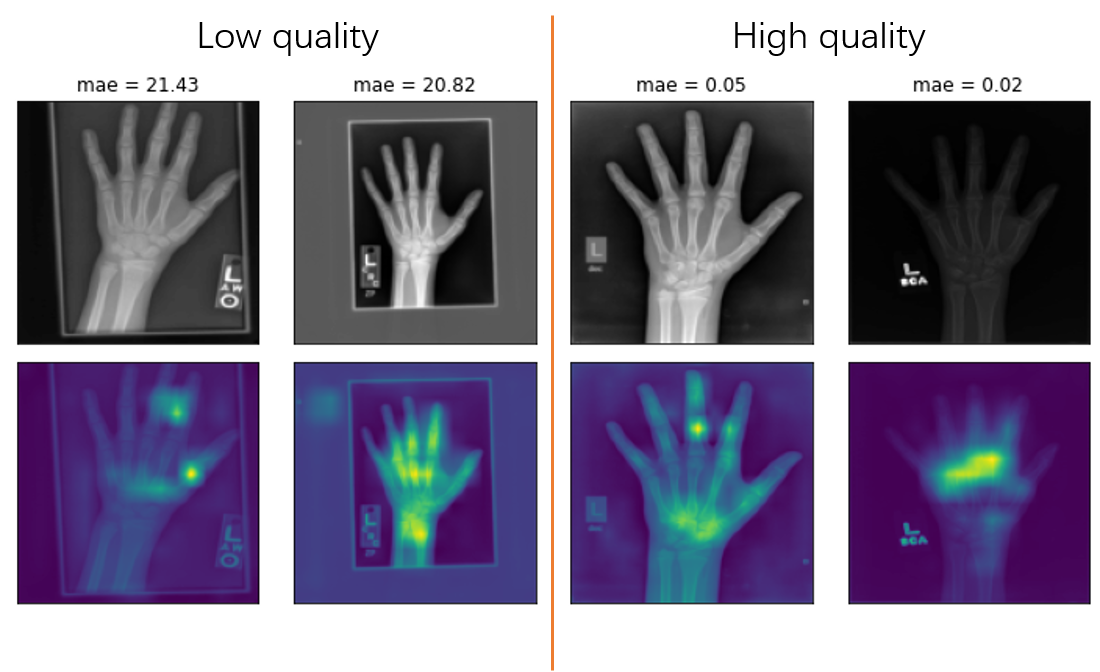
\includegraphics[width=8.5cm]{cam.png}}
%  \vspace{2.0cm}
\end{minipage}
%
%
\caption{First row is the hand X-ray image.The second row is the saliency map based on grad-cam.A high quality saliency map(low MAE) usually clearly highlight one or two parts of hand.}
\label{fig:res}
%
\end{figure}
% Below is an example of how to insert images. Delete the ``\vspace'' line,
% uncomment the preceding line ``\centerline...'' and replace ``imageX.ps''
% with a suitable PostScript file name.
% -------------------------------------------------------------------------
\begin{figure*}[t]

\begin{minipage}[b]{1.0\linewidth}
  \centering
  \centerline{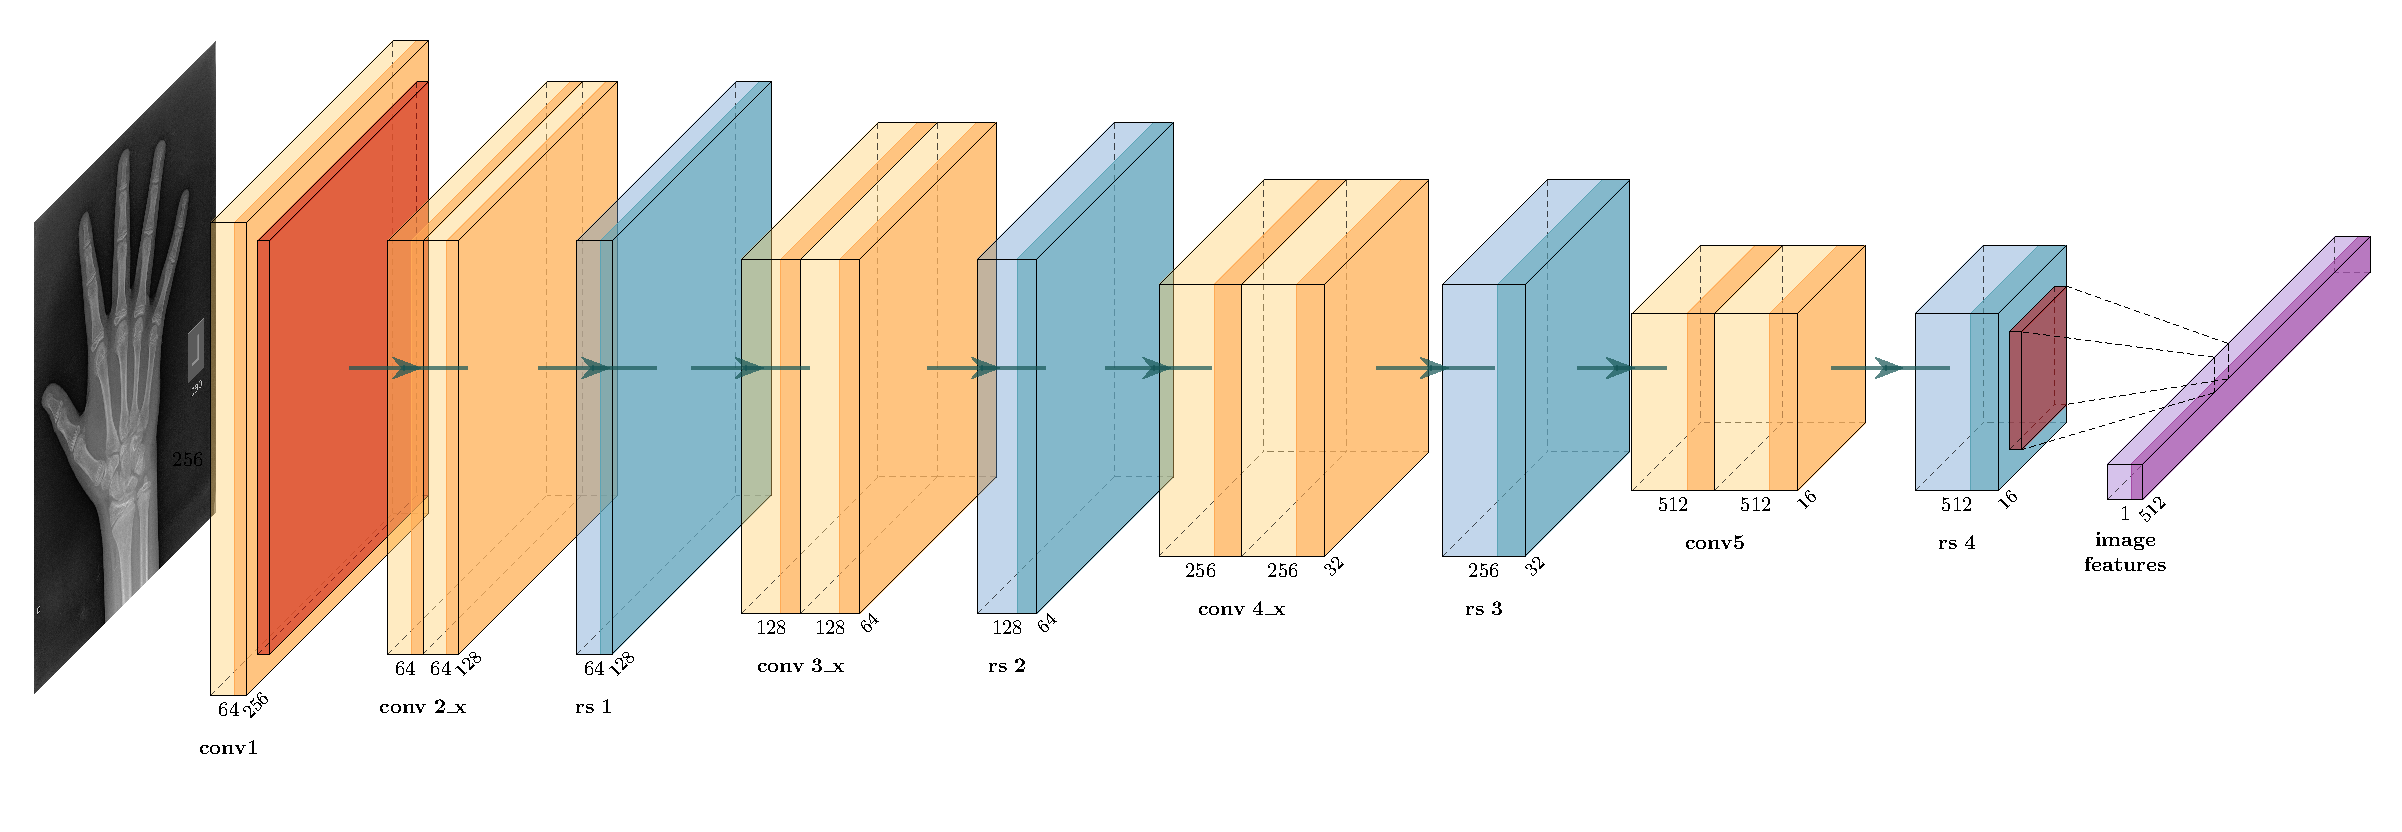
\includegraphics[width=12cm]{RS_Resnet18.pdf}}
%  \vspace{2.0cm}
  \centerline{(a) Whole strucuture of RSAnet18}\medskip
\end{minipage}
%
\begin{minipage}[b]{.32\linewidth}
  \centering
  \centerline{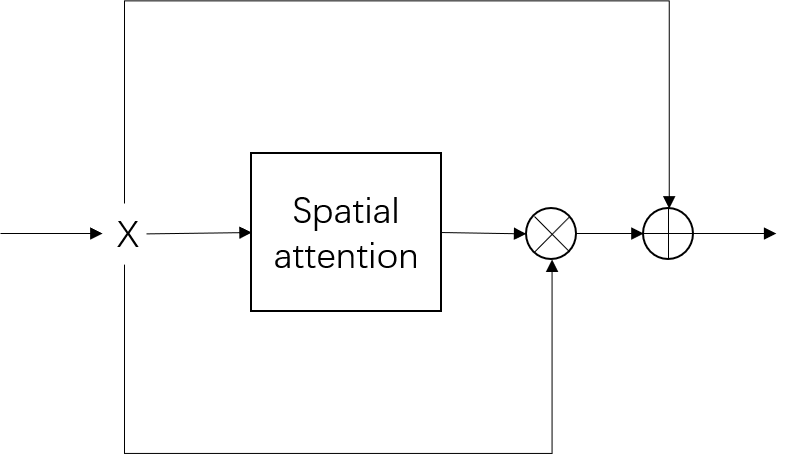
\includegraphics[width=5.5cm, height=3.5cm]{r_attention.png}}
%  \vspace{1.5cm}
  \centerline{(b) RSA module}\medskip
\end{minipage}
\begin{minipage}[b]{.32\linewidth}
  \centering
  \centerline{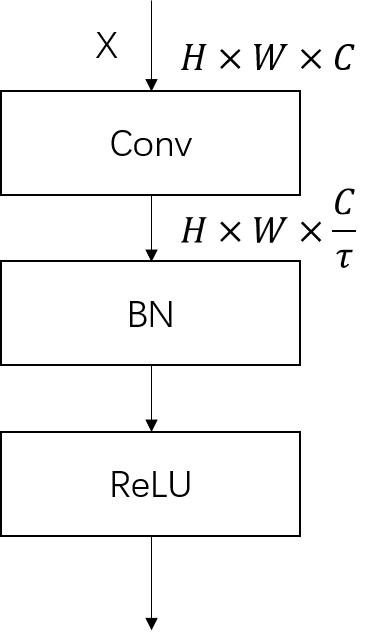
\includegraphics[width=2.5cm,  height=4.0cm]{rd.png}}
%  \vspace{1.5cm}
  \centerline{(c)  dimensionality reduction module}\medskip
\end{minipage}
\begin{minipage}[b]{0.32\linewidth}
  \centering
  \centerline{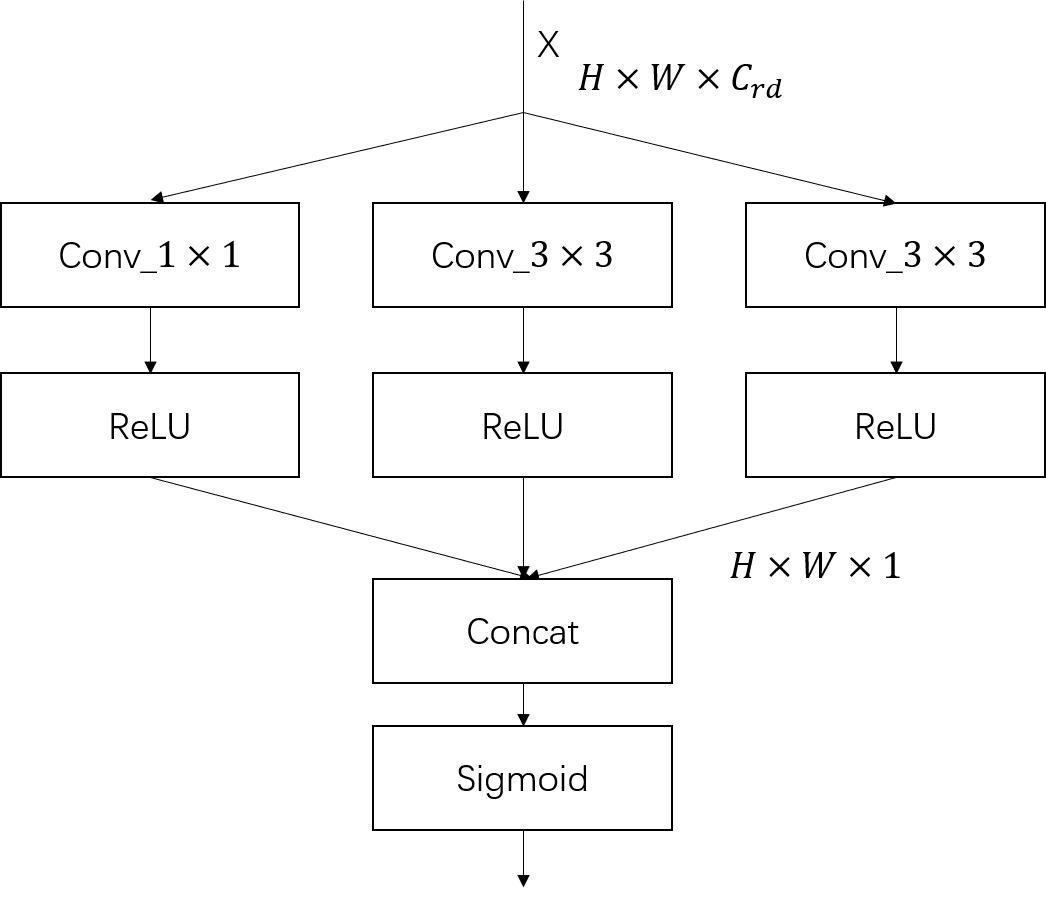
\includegraphics[width=4.5cm,  height=4.5cm]{attention.png}}
%  \vspace{1.5cm}
  \centerline{(d) multi-scale-head attention}\medskip
\end{minipage}
%
\caption{In (a),behind each convolution block, there is an RSA module.The RSA module strucutre shown by (b), which consisted of dimensionality reduction module(c) and multi-scale-head attention(d)}
\label{fig:res}
%
\end{figure*} 
A more effective residual spatial attention module structure proposed in our work. We improve the spatial attention from two different perspectives: module depth and kernel size. Both will be discussed in more details in the later sections. Compared with PRSNet\cite{ji2019prsnet}, the residual attention structure is simplified to alleviate overfitting and a "multi scale head" attention, inspired by inception structure\cite{szegedy2016rethinking} and multi-Head attention\cite{vaswani2017attention}, is proposed to enables the spatial attention to considers different scale information. In addition, different degrees of dimensionality reduction refer from senet\cite{hu2018squeeze} is used to reduce the difficulty of learning spatial attention, and to a certain extent, further reduce the risk of overfitting. Our module enables each level of the feature maps to learn an independent spatial attention rather than putting spatial attention modules at the end of the network, like the structure proposed by Wu et.al\cite{wu2019residual}. Because spatial attention helps the following convolutional layer to extract higher quality features. Our method outperforms all state-of-the-art models with a single branch structure in the dataset of RSNA Pediatric Boneage Age Chanllenge(2017).



\section{METHODOLOGY}
\label{sec:format}
In the following sub-sections, the details of the whole structure(Fig.2 (a)) and residual spatial attention module(Fig.2 (b)) are presented.
\subsection{Macro structure}
\label{ssec:subhead1}
As Fig.1 illustrated, learning of the spatial attention is the major challenge and the texture features are relatively simple to be learnt. Our experiments have shown that spatial attention has zero tolerance for the redundancy of the network structure. Increasing complexity of network structure raise the difficulty of training and amplify the risk of overfitting. Therefore the resnet34 and resnet50\cite{he2016deep}, which are most suitable for BAA task, are employed as backbone.

For the task of BAA, higher input images resolution enable CNN to extract more important details which significantly improves the prediction results. However, this lead to the increase size of feature maps outputted by CNN which cause more information to be lost after global average pooling (GAP). Adding a spatial attention block before the final GAP layer can be considered as assigning different weights to the GAP kernel such that the uncontributed regions are ignored and alleviate information compression. In addition, some attempts about adding spatial attention block separately between different convolution blocks demonstrate that the MAE inserted behind conv\_4 is far better than added after last block(conv\_5). This means that it is also very important to introduce spatial attention between the convolutional blocks, which can make the convolutional layer at the [back] concentrate on important areas and extract effective texture features more effectively.Therefore, the Residual spatial attention blocks are inserted behind each level of blocks(conv 2\_x to conv 5\_x) as Fig.2 shown.

% \begin{table*}[!htbp]
% \begin{minipage}[b]{1.0\linewidth}
%   \centering
% \begin{tabular}{|c|c|c}
% \hline
% RSA module name  & RSAnet 34 & RSAnet 50 \\
% \hline
% ras1 &  \tabincell{c}{dim\_reduce(16), 4\\ multi\_scale\_attention()} & \tabincell{c}{dim\_reduce(16), 16\\ multi\_scale\_attention()}\\
% \hline
% ras2  &  \tabincell{c}{dim\_reduce(16), 8\\ multi\_scale\_attention()} & \tabincell{c}{dim\_reduce(4), 128\\ dim\_reduce(8), 16\\ multi\_scale\_attention()}\\
% \hline
% ras3  &  \tabincell{c}{dim\_reduce(16), 16\\ multi\_scale\_attention()} & \tabincell{c}{dim\_reduce(8), 128\\ dim\_reduce(8), 16\\ multi\_scale\_attention()}\\
% \hline
% ras4  &  \tabincell{c}{dim\_reduce(16), 32\\ multi\_scale\_attention()} & \tabincell{c}{dim\_reduce(8), 256\\ dim\_reduce(16), 16\\ multi\_scale\_attention()}\\
% \hline
% \end{tabular}
% \end{minipage}
% \caption{The dim\_reduce(x) is the dimensionality reduction module, and the x is the reduction factor. the left number is the number of channels. multi\_scale\_attention indicates the multi-scale attention module.}
% \end{table*}

\begin{table}[!htbp]
\begin{minipage}[b]{1.0\linewidth}
  \centering
\begin{tabular}{|c|c|c|}
\hline
RSA module name  & RSAnet 34 & RSAnet 50 \\
\hline
ras1 &  \tabincell{c}{DR(16), 4\\ MSA()} & \tabincell{c}{DR(16), 16\\ MSA()}\\
\hline
ras2  &  \tabincell{c}{DR(16), 8\\ MSA()} & \tabincell{c}{DR(4), 128\\ DR(8), 16\\ MSA()}\\
\hline
ras3  &  \tabincell{c}{DR(16), 16\\ MSA()} & \tabincell{c}{DR(8), 128\\ DR(8), 16\\ MSA()}\\
\hline
ras4  &  \tabincell{c}{DR(16), 32\\ MSA()} & \tabincell{c}{DR(8), 256\\ DR(16), 16\\ MSA()}\\
\hline
\end{tabular}
\end{minipage}
\caption{The DR(x) is the dimensionality reduction module, and the x is the reduction factor. the left number is the number of channels. MSA() indicates the multi-scale attention module.}
\end{table}

\subsection{Residual spatial attention block}
\label{ssec:subhead2}
\textbf{Residual structure:} Adding a simple spatial attention block to each convolution block is not as [expected], but the MAE loss is significantly increased. The behavior is due to a high repeatability among the various spatial attention blocks and it leads to severe overfitting. The residual structure is introduced to solve this problem. It allows the spatial attention blocks to establish a good cooperative relationship. The global spatial relationship is learned through the last block and each block in front only learns an attention map to assist the next  convolutional block for feature extraction. In addition,different convolutional blocks have different requirements for spatial attention. The skip connnection can exert a weak influence on blocks that are not sensitive to spatial attention.Given the input feature map. 
$x_{i}$
The corresponding attention  mapping is
$RSA_{i}(x_{i})$ 
is produced by a list of convolutional operations, then the output for each spatial attention model is  
$$
x_{i} = x_{i}*RSA_{i}(x_{i}) + x_{i}
$$

\textbf{Spatial attention generator:} The attention generator is consisted of two parts, dimensionality reduction module and different scale heads attention module(Fig.2 (c) and Fig.2(d)).
Initially, we just apply $1\times1$ convolution to produce attention map, however, when we separately add the spatial attention module to a certain convolution block, we find that if the number of input channels is more than 256, the network cannot learn the correct attention. In order to tackle this issue, a extra $1\times 1$ convolution block is utilized to reduce the number of channels of the input feature map to $\frac{1}{\gamma}$. On the one hand, this can be regarded as a method of reducing the dimensionality. The important part of the input feature map is extracted through convolution and mapped to $\frac{1}{\gamma}$ dimensions to reduce the complexity of training. [On the other hand], this can be considered as increasing the performance of the attention module by increasing the depth. For the number of feature map channels [is greater] than 512, cascading two dimensionality reduction modules leads to a lower MAE loss, therefore, there are two dimensionality reduction module  in all residual attention module of RSAnet 50 except the rsa\_1.
The different scale heads attention module is connected after the dimensionality reduction module. It learns the attention maps of different receptive fields through three sets of different size convolution kernels($1\times 1$, $3\times 3$, $5\times 5$), and then use one convolution to achieve the weighted summation of the three attention maps,finally, input it into the Sigmoid function to map the result into a probability map. The original intention of this module was designed to make the attention module not only consider the importance of the current position, but also consider the relationship between adjacent elements. This is particularly important for the attention module between the two convolutional blocks, which enables the attention module to analyze the structure of the texture more macroscopically, predict the demand of the convolution module behind, and give the attention comprehensively. In order to be compatible with the needs of different convolution modules, the weight of the attention of different receptive fields is automatically learned through a $1\times1$convolution.

\subsection{Corresponding data augmentation}
\label{ssec:subhead3}

Because of the vulnerability and higher risk of overfitting, some [specific] data augmentation methods, Random erasing\cite{zhong2020random} and Random Cropping, are indispensable. Random erasing is used to erase a rectangulair area randomly and fill it with 0, so that the network are still able to predict the accurate result depends on the remaining part. It is a effective approach to reduce the dependence on a specific area for attention module. For Random cropping,it not only reduces the dependence of the addition module on the special area, but also reduces its sensitivity to position and size. They are the guarantee of learning an effective and robust spatial attention.

\section{EXPERIMENTS}
\label{sec:pagestyle}
\textbf{Dataset, pre-processing and traning details:}
Our model is evaluated by the dataset of RSNA Pediatric Bone age Age Chanllenge(2017), including 12611 X-ray image in training set and 200 images in test set. Besides two crucial augmentations, random erasing and random cropping, the affine transform(shifting, scaling, rotation), horizontal flipping, random brightness and contrast are applied. We utilize all eight cores of TPU V2 for distributed training with ADAM optimizer in 100 epochs, for each mini-batch of RSAnet18 and RSAnet34 consisted of 256 $512\times512$ X-ray images and the batch size of RSAnet50 is 128. The initial learning rate is 5e-5. Every 10 epoches and the learning rate decay to half. All our results have used mean Absolute Error(MAE) as the criterion, a smaller score means higher performance

\textbf{Baseline:}The baseline uses the same strategy as the winning solution of RSNA 2017 challenge, except for the backbone of se-resnet152. The reason is se-resnet152 outperforms other structure and achieves 5.58 MAE in testset. Moreover, we want to show an intuitive contrast about the performance of channel-wised attention and spatial-wised attention for Bone age assessment.

\textbf{Result and Comparison with State-of-the-Arts:}The RSAnet50 achieved the best result, MAE of 4.51 in test set,  which is the first single branch model under 4.5(MAE).The MAE of RSAnet34 is (4.69).

\begin{table}[!htbp]
\begin{minipage}[b]{1.0\linewidth}
  \centering
\begin{tabular}{c|c|c|c}
\hline
Method & Baseline & RSAnet 34 & RSAnet 50 \\
\hline
MAE & 5.58 & 4.69 & 4.51\\
\hline
\end{tabular}
\end{minipage}

\end{table}


\begin{figure}[htb]

\begin{minipage}[b]{1.0\linewidth}
  \centering
  \centerline{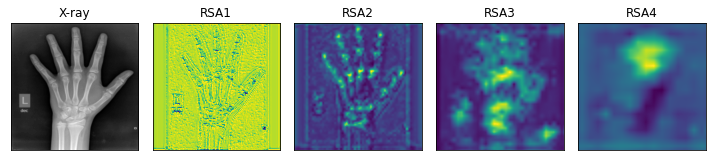
\includegraphics[width=8.5cm]{result.png}}
%  \vspace{2.0cm}
\end{minipage}
%
%
\caption{The attention map for each RSA module in RSAnet34.The input X-ray image is on the left.}
\label{fig:res}
%
\end{figure}
In Fig.3 For this X-ray image, the RSA1 block basically learn the outline attetnion, and both RSA1 and RSA2 block learn some important area information.The last RSA did not learn much useful information,one possible reason is features are over-enhanced by the first few attention modules to  facilitate feature extraction, and the last module needs to suppress some unimportant parts.
\section{CONCLUSIONS}
\label{sec:typestyle}
In this study, a novel structure based on spatial attention is proposed. The spatial attention module is optimized from position, residual structure, depth, width and diversity of convolution kernel. The effectiveness has already demonstrated and the performance achieves state-of-the-art and outperforms other public benchmarks of single branch models. Furthermore, our model can generalize to general classification or detection task. In the future, we will try to further upgrade the spatial attention structure on some general data sets and incorporate channel-wised attention.


\bibliographystyle{IEEEbib}
\bibliography{refs}

\end{document}
